\documentclass{cookedoc}
\copyrightyear{2017}
\pubyear{2017}
\usepackage{upgreek}
\usepackage{mathtools}
\usepackage{natbib}
\usepackage{graphicx}
\usepackage{grffile}
\usepackage{float}
\usepackage{listings}
\usepackage{color}
\usepackage{enumerate}
\setlength{\parindent}{0pt}
\setlength{\parskip}{1em}
\setlength{\belowcaptionskip}{0pt}

\definecolor{dkgreen}{rgb}{0,0.6,0}
\definecolor{gray}{rgb}{0.5,0.5,0.5}
\definecolor{mauve}{rgb}{0.58,0,0.82}

\lstset{frame=tb,
	language=C++,
	aboveskip=3mm,
	belowskip=3mm,
	showstringspaces=false,
	columns=flexible,
	basicstyle={\small\ttfamily},
	numbers=none,
	numberstyle=\tiny\color{gray},
	keywordstyle=\color{blue},
	commentstyle=\color{dkgreen},
	stringstyle=\color{mauve},
	breaklines=true,
	breakatwhitespace=true,
	tabsize=3
}

\begin{document}
	\firstpage{1}
	\onecolumn
	
	\title{\Large Y4 project proposal - To Validate The Use of Deep Learning To Predict 3D Objects With Deformations From a 2D STEM Image.}
	\author{\large Ziyue Wang}
	
	\address{Supervisor Dr Wolfgang Theis}
	\history{\normalsize 26/10/2018}
	\editor{\bf{Keywords:} \rm SOC, Forest fire, Mean-field theory, }
	
	
	\maketitle
	\section{Abstract}
	
	\section{Introduction}
	
	In the past decade Scanning Transmission Electron Microscopy (STEM) has become an extremely useful tool, with the ability of resolving images of multiple material classes from semiconductors to superconductors (ref). They have also been used to probe the chirality of materials (Smith, Scott Graeme 2017), observing systems such as a simple hexagonal helix. STEM is also a very useful tool in imaging biological specimens in the nano-regime; Three-dimensional reconstructions of cytoskeleton and calthrin-coated pit in mammalian cells have been performed using STEM (Jonge et al 2010). 
	
	As a result of the rapid development of STEM and other electron microscopies (such as transmission electron tomography(TEM) or scanning electron tomography (SEM)), a characteristic aspect of these techniques is the large volume of experimental data as either static or dynamic images. Although electron microscopy techniques provide an immediate view into the atomic structures, analysis of the structure and deformations requires much manual work. Analysis on image sequences proves to be even more problematic as factors such as small rotations, vibrations, thermal drift may modify the image over time. 
	
	There has been significant improves in machine learning for image classification in the past few years, with deep learning being the centerpiece of it all. The increased data available for training has been the major reason for the popularity of deep learning, as the multitude of training data pushed neural networks to be more precise and accurate than ever before. The rise came in 2012, as records were broken by a deep learning algorithim in an online image classification contest called the ImageNet Challenge. Since then, the number of deep learning publications has almost doubled from 2008 to 2016 ), increasing every year up to then, with 2017 on-track to be the highest yet (over 12,000 publications within half a year) (Amir Mosavi 2018). Convolutional neural networks (CNNs) has been consistenly excellent in visual recognition tasks, ranging from automated segmentation of brain images (T.M.Quan 2016) to particle detection from cryo-electron microscopy images (Y.zhu et.al 2017). 
	
	A neural network trained on STEM images can bring many advantages to nanoscience researches such as: (i) automated image classification, which would remove any manual classification all together; (ii) a database which allows researches to find specific categories of STEM images; (iii) Extraction of images for future tasks which require a specific class, such as in the mass-production of catalysts which require optimized nanoparticles. 
	
	There has been past publications which have had success in the classification of EM images. Modarres et.al (2017) used transfer learning on a previously trained 
	CNN, using a set of ~20,000 manually classified SEM images. Dyck et.al (2017) also had similar success, instead choosing to build a fully convolutional network (FCN) from scractch, using an autoencoder system with learning filters at every layer and training the network using simulated images. However, the group only trained the network to identify single layers of atoms, which is effectively a 2D structure. Deep learning with HRTEM images has also been accomplished (Madsen et.al 2018), whom used a similar approach to Dyck (2017). 
	
	Automated analysis using deep learning on fully 3D structures from STEM images has yet to be attempted. This project proposes to do just that, and to compare the efficacy of transfer learning with building a series of neural networks from scratch. The network should be compatible with STEM images obtained experimentally, aiding in the eventual classification of fully 3D chemical and atomic structures. 
	
	\section{Aims}
	
	The main objective of this project is to be able to classify objects through STEM imaging while detecting deformations, in an automated way. In the grand scheme of things, this would be expanded to classify experimental images taken using a STEM microscope. The more specific aims I want to achieve through this project are:
	
	\begin{enumerate}
		\item   Build a fully functional simulation of which STEM images can be produced of 3D objects with varying dimensions. The simulation should a`lso be able to simulate experimental data.
		\item   A CNN (convolutional neural network) capable of detecting fully 3D object from STEM images, transfer trained using a previously trained network.
		\item   A system of multiple neural networks: One to detect image outlines, depth detection e.t.c, another to identify the object from the information extracted from the previous.
		\item   A neural network that can find the "ground truth" of an object's classification from experimental data, trained using simulated experimental data. 
		
	\end{enumerate}
	\section{Literature review}
	
	Krizhevsky et.al (2012) trained a deep convolutional neural network (deep CNN) to classify over 1.2 million images that was presented in the 2012 ImageNet online contest. With deep learning they were able to win the competition with the lowest error rate to date, beating the second place team by over $10\%$. The overall network consisted of 8 layers, first five are CNN and last three are FCN. Output is fed to a 1000-way softmax which in turn has 1000 class labels.	
	
	In Annular Dark-field Scanning Transmission Electron Microscopy (ADF-STEM), it has been shown that the detector collects scattered electrons obeying the Rutherford scattering, which is proportional to $Z^2$, but realistically is $Z^{1.5-1.8}$ (ref33 in STEM paper). The probability of multiple scatters scales linearly (page 28, TEM for material science), so the thickness of a sample can be calculated through direct integration. 	(STEM paper ref) added random noise and blurring in the ranges comparible to those typically observed in experimentation. The scan noise/distortion is expected to be $~5\%$ and shot noise $<1\%$, due to enviromentally instability and poisson noise respectively (L jones 2015, quantitatve ADF STEM: acquisition....). The latter scales with $1/\sqrt{dose}$. 
	
	Talk about the 3 papers and that masters thesis we found.
	
	
	
	
	
	\section{Expected results}
	
	The expected result is to have a neural network which is capable of classifying 3D STEM images with $~80\% +$ accuracy. 3D structures of varying dimensions, orientations and deformations should be distinguishable from other structures. A searchable database of each of the images shall be readily available for further work. 
	
	
	
	\section{Methods and management}
	
	A proposed schedule can be found below in fig.(\ref{GANT}) in the form of a GANT chart. It is color-coordinated: Green indicated the basic (and hence most important) tasks, blue indicates the extension tasks and red is deadline periods/dates. Grid/dashed either indicate additional time and holidays. The extension tasks will only be attempted once the basic tasks have been completed. 
	
	\begin{figure} [H]
		\centering
		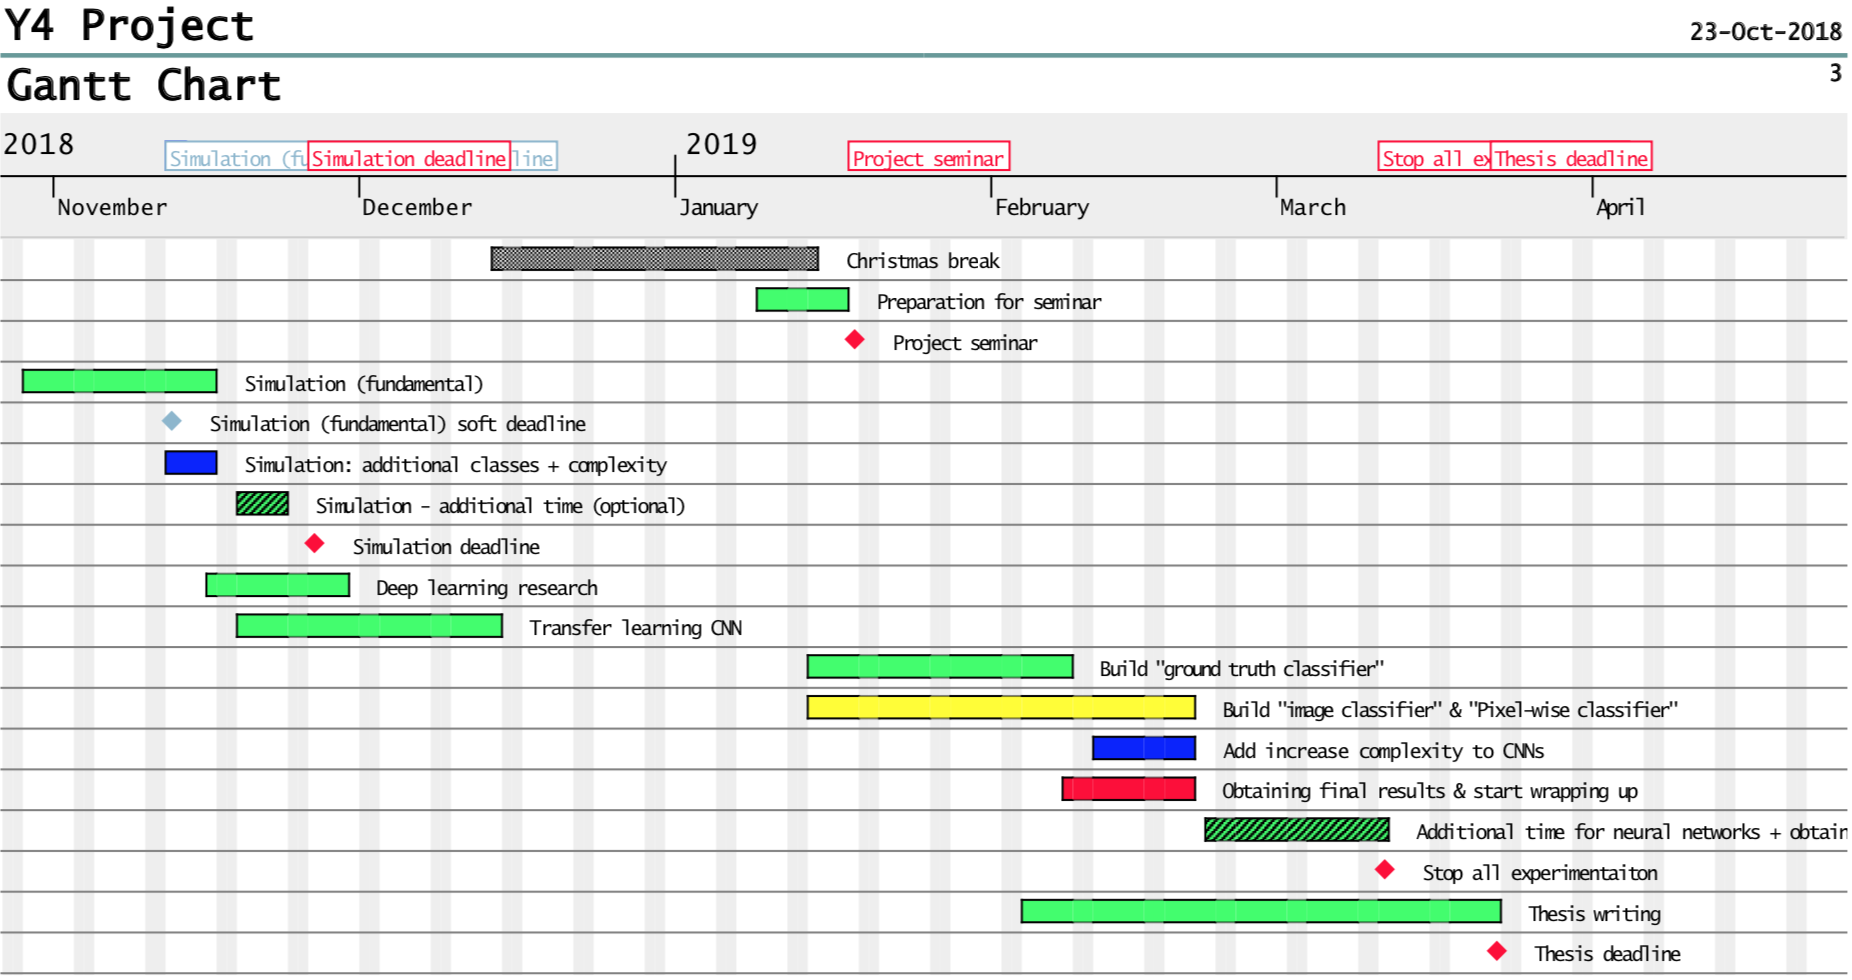
\includegraphics[width=\linewidth]{gant2.png}
		\caption{GANT chart of the timeline proposed for this project. Each task is explained later on.}
		\label{GANT}
	\end{figure} 
	
	For the simulation, I will implement Object Orientated Programming (OOP) in python, making use of the readily available libraries to simulate STEM images. Annular dark field imaging will be used alongside direct integration of the object structure to produce our image. The fundamental components of the simulation will include: noise implementation image and deformations of the structure, multiple structures (sphere, cube, rectangle e.t.c), varying dimensions (larger and smaller shapes), and lastly varying orientations. Artificial noise will be based on the detector imperfections. Poisson noise (scailing with 1/$\sqrt dose$) and distortion (frequency and dwell-time-dependent) of $~5\%$ will be introduced as it is a uncontrollable factor of the machinary. 
	
	 Extensions to this programme will include but not limited to: more similar shapes (i.e. cones and pyramids), movement of objects through the imaging period, and lastly the ability to simulate experimental data (additional noise e.t.c). 
	
	The first network I will attempt to implement is one that has be trained through transfer learning. I plan on taking previously trained CNNs (Inception-v3, inception-v4) alongside the TensorFlow (TF) library, only retraining the last layer of the CNN with my simulated images. This network will be referred to as the Transfer Learnt Image Classifier (TLIC) and it will attempt to classify the structure from a single STEM image. If this proves to be unsuccessful before the Christmas holidays, I will attempt to build my own set of CNNs to classify the images. The first CNN, named the "Pixel-wise classifier", will attempt to simplify STEM images by detecting and extracting the boundaries and volumes of each structure. The second will attempt to classify the images "Image Classifier", taking information from the first CNN, using a "weakly supervised" algorithm, and use this to compare against the classification results from the transfer learning algorithm. 
	
	If the transfer learning network is capable of classifying images with relatively low errors, I will instead move straight on to write a "ground truth" classifier. This classifier will also make use of transfer learning onto previously trained CNNs alongside TF libraries, and trained with simulated experimental data produced from the simulation. The main difference would be to adapt this network to find the "ground truth" classification of the structure from multiple images, rather than attempting to classify the structure from a single image. If the transfer learning was unsuccessful however, I will attempt to build this from scratch, like the "Pixel-wise Classifier" and the "Image Classifier". This network is required for a fluid workflow for future experimental use, as the ground truth will not be known at the time of experimentation. 
	
	If building my own classifier CNN fails while transfer learning is achievable, I will abandon that and focus on improving the transfer learning CNN by providing it with more rigorous training data and additional other networks to transfer train.
	
	The ground truth classifier should be attempted as soon as a working deep learning network for classifying simulated data has been achieved. This is so that there can be a streamlined work flow for future work pertaining to image classification, especially if data is taken experimentally with no known ground truth. The pixel-wise classifier may need to be build simultaneously with this in order to reach deadlines. 
	
	
	\section*{Acknowledgements}
	%ENTER ACKNOWLEDGEMENTS TEXT BELOW
	
	\section*{Reference}
	
	
\end{document}
